\documentclass[conference]{IEEEtran}

\IEEEoverridecommandlockouts

\usepackage{cite}
\usepackage{amsmath,amssymb,amsfonts}
\usepackage{algorithmic}
\usepackage{graphicx}
\usepackage{textcomp}
\usepackage{xcolor}
\usepackage{hyperref}


\begin{document}

\title{Implementation of an email-based alert system for large-scale system resources}

\author{\IEEEauthorblockN{Robert Poenaru$^{1,2}$}
\IEEEauthorblockA{
%$^{1}$Department of Computational Physics and Information Technology\\ 
$^{1}$\textit{Horia Hulubei} National Institute of Nuclear Physics and Engineering, Magurele, Romania\\
$^2$Doctoral School of Physics, University of Bucharest, Romania\\
robert.poenaru@nipne.ro}
}

\maketitle

\begin{abstract}
Tackling the current problems of interest for physicists that deal with various topics require lots of computing simulations. Identifying and preventing any unusual behavior within the system resources that execute large-scale calculations is a crucial process when dealing with system administration, since it can improve the run-time performance of the resources themselves and also help the physicists by obtaining the required results faster. In the present work, a simple \emph{pythonic} implementation which 1) monitors a given computing architecture (i.e., its system resources such as CPU and Memory usage), and 2) alerts a custom team of administrators via e-mail in almost real-time when certain thresholds are passed, is presented. Using existing packages written in Python, with the current implementation it is possible to send e-mails to a predefined list of clients containing detailed information about any machine running outside the "normal" parameters.
\end{abstract}

\begin{IEEEkeywords}
python, system resources, alerting, email, smtp, monitoring, watchdog
\end{IEEEkeywords}

\section{Introduction}

The computing resources within a physics department must be up to speed and ready for a continuous run-time of small-, medium-, but also large-scale simulations, in order to assure a consistent and optimal workflow for the research teams that require calculations. Usually, there is a cohesive workflow between the scientists that want to run their simulations and the system administration (sysadmins) team that provides the necessary resources for executing them. The sysadmins must check that the resources which are performing calculations behave well, but they must also take care of the computing equipment that is sitting in \emph{idle}-mode, in case new requests for allocating resources are issued by scientists. The process of resource management is crucial since it involves many factors in deciding which are the most optimal compute nodes that could start a new job, in terms of efficiency and speedup \cite{paya2015resource}, these being deciding factors in the total run-time of the simulations themselves.
\par Proper job allocation, management, and execution will result in minimal impact of resource slowdown, process blocking, or even dead-locks in the executing pipeline, giving the possibility of the researchers to obtain the desired numerical results in as fast as possible. 
\par On the other hand, any code optimization \cite{codeoptimization2,codeoptimization1} on the submitted simulations (done exclusively by the scientific teams) will also take advantage of the allocated resources, since \emph{better code} implies faster execution, lower impact on the memory pool and much lower probability of program interruption.
\par One can conclude that indeed, better resource management (done by the sysadmins) will result in better code execution, helping thus the scientists, but in the same way, any code optimization made by scientists will help the sysadmins, since the degree of failure within the executing simulations stack could be decreased. This reciprocal-mode of improvements (for both \emph{communities}) is sketched in Fig. \ref{community-optimization}, where the key characteristics of both \emph{communities} (i.e., physicists issuing simulations and sysadmins dealing with computing management) are emphasized. The arrows signify the \emph{reciprocal improvement cycle} between the two.
\par However, due to the large degree of complexity of the underlying computing infrastructure, issues related to memory bandwidth, network stability, CPU throttling \cite{ibm}, cache availability \cite{awscache} and so on are highly probable, especially when the machines are running continuously. Frequent updates, unexpected network traffic, errors within the services running in the application layer \cite{pstree} could also affect the idling nodes. While the former issues will only affect the simulations that are currently being executed, the latter set of issues could produce unexpected delays in the starting process of the job queue \cite{jobqeue}, which will increase the wait-time of simulation results. One can see that indeed, any issues which occur with the computing resources, even the idling ones, can affect the workflow of the research teams, causing the entire research department to finish their projects. As such, the sysadmins are essential by taking the proper actions on the computing infrastructure.
\par Unfortunately, there will always be moments when the sysadmin team that is monitoring a particular computing node (e.g., cluster, server racks, etc.) cannot keep track of the \emph{health status} of the entire architecture at all times (although recently, some interesting models emerged within the literature that could improve the machine health status \cite{hasani2019machine,lin2020health} in an automated way). 

\begin{figure}[htbp]
\centerline{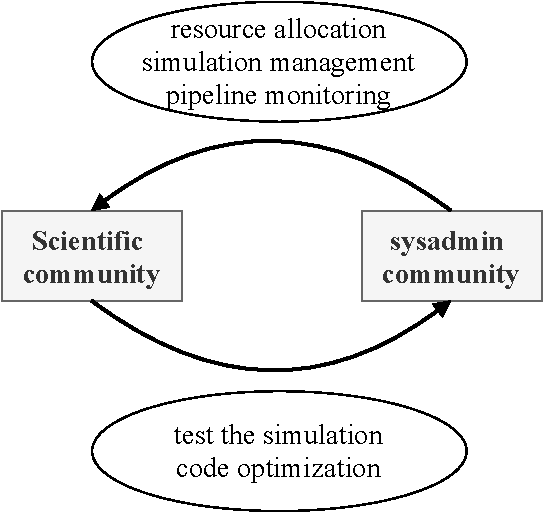
\includegraphics[scale=0.7]{figs/scientific_sysadmin_optimization.pdf}}
\caption{A basic relationship between the scientific community that issues simulations to be executed on the computing resources, and the system administration team that deals with process allocation, execution and management of resources.}
\label{community-optimization}
\end{figure}



% \subsection{Figures and Tables}
% \paragraph{Positioning Figures and Tables} Place figures and tables at the top and 
% bottom of columns. Avoid placing them in the middle of columns. Large 
% figures and tables may span across both columns. Figure captions should be 
% below the figures; table heads should appear above the tables. Insert 
% figures and tables after they are cited in the text. Use the abbreviation 
% ``Fig.~\ref{fig}'', even at the beginning of a sentence.
% \begin{table}[htbp]
% \caption{Table Type Styles}
% \begin{center}
% \begin{tabular}{|c|c|c|c|}
% \hline
% \textbf{Table}&\multicolumn{3}{|c|}{\textbf{Table Column Head}} \\
% \cline{2-4} 
% \textbf{Head} & \textbf{\textit{Table column subhead}}& \textbf{\textit{Subhead}}& \textbf{\textit{Subhead}} \\
% \hline
% copy& More table copy$^{\mathrm{a}}$& &  \\
% \hline
% \multicolumn{4}{l}{$^{\mathrm{a}}$Sample of a Table footnote.}
% \end{tabular}
% \label{tab1}
% \end{center}
% \end{table}

\section*{Acknowledgment}

This work was possible through the Department of Computational Physics and Information Technology at \emph{Horia Hulubei} National Institute of Physics and Nuclear Engineering.

\bibliographystyle{unsrt}

\bibliography{references}

\end{document}
